
\documentclass[border=10pt, 12pt]{standalone}
\usepackage[svgnames]{xcolor}
\usepackage{amsmath}
\usepackage{pgfplots}
\pgfplotsset{compat=newest}
\usepackage[sfdefault]{FiraSans}
\usepackage{FiraMono}
\renewcommand*\familydefault{\sfdefault}
\begin{document}
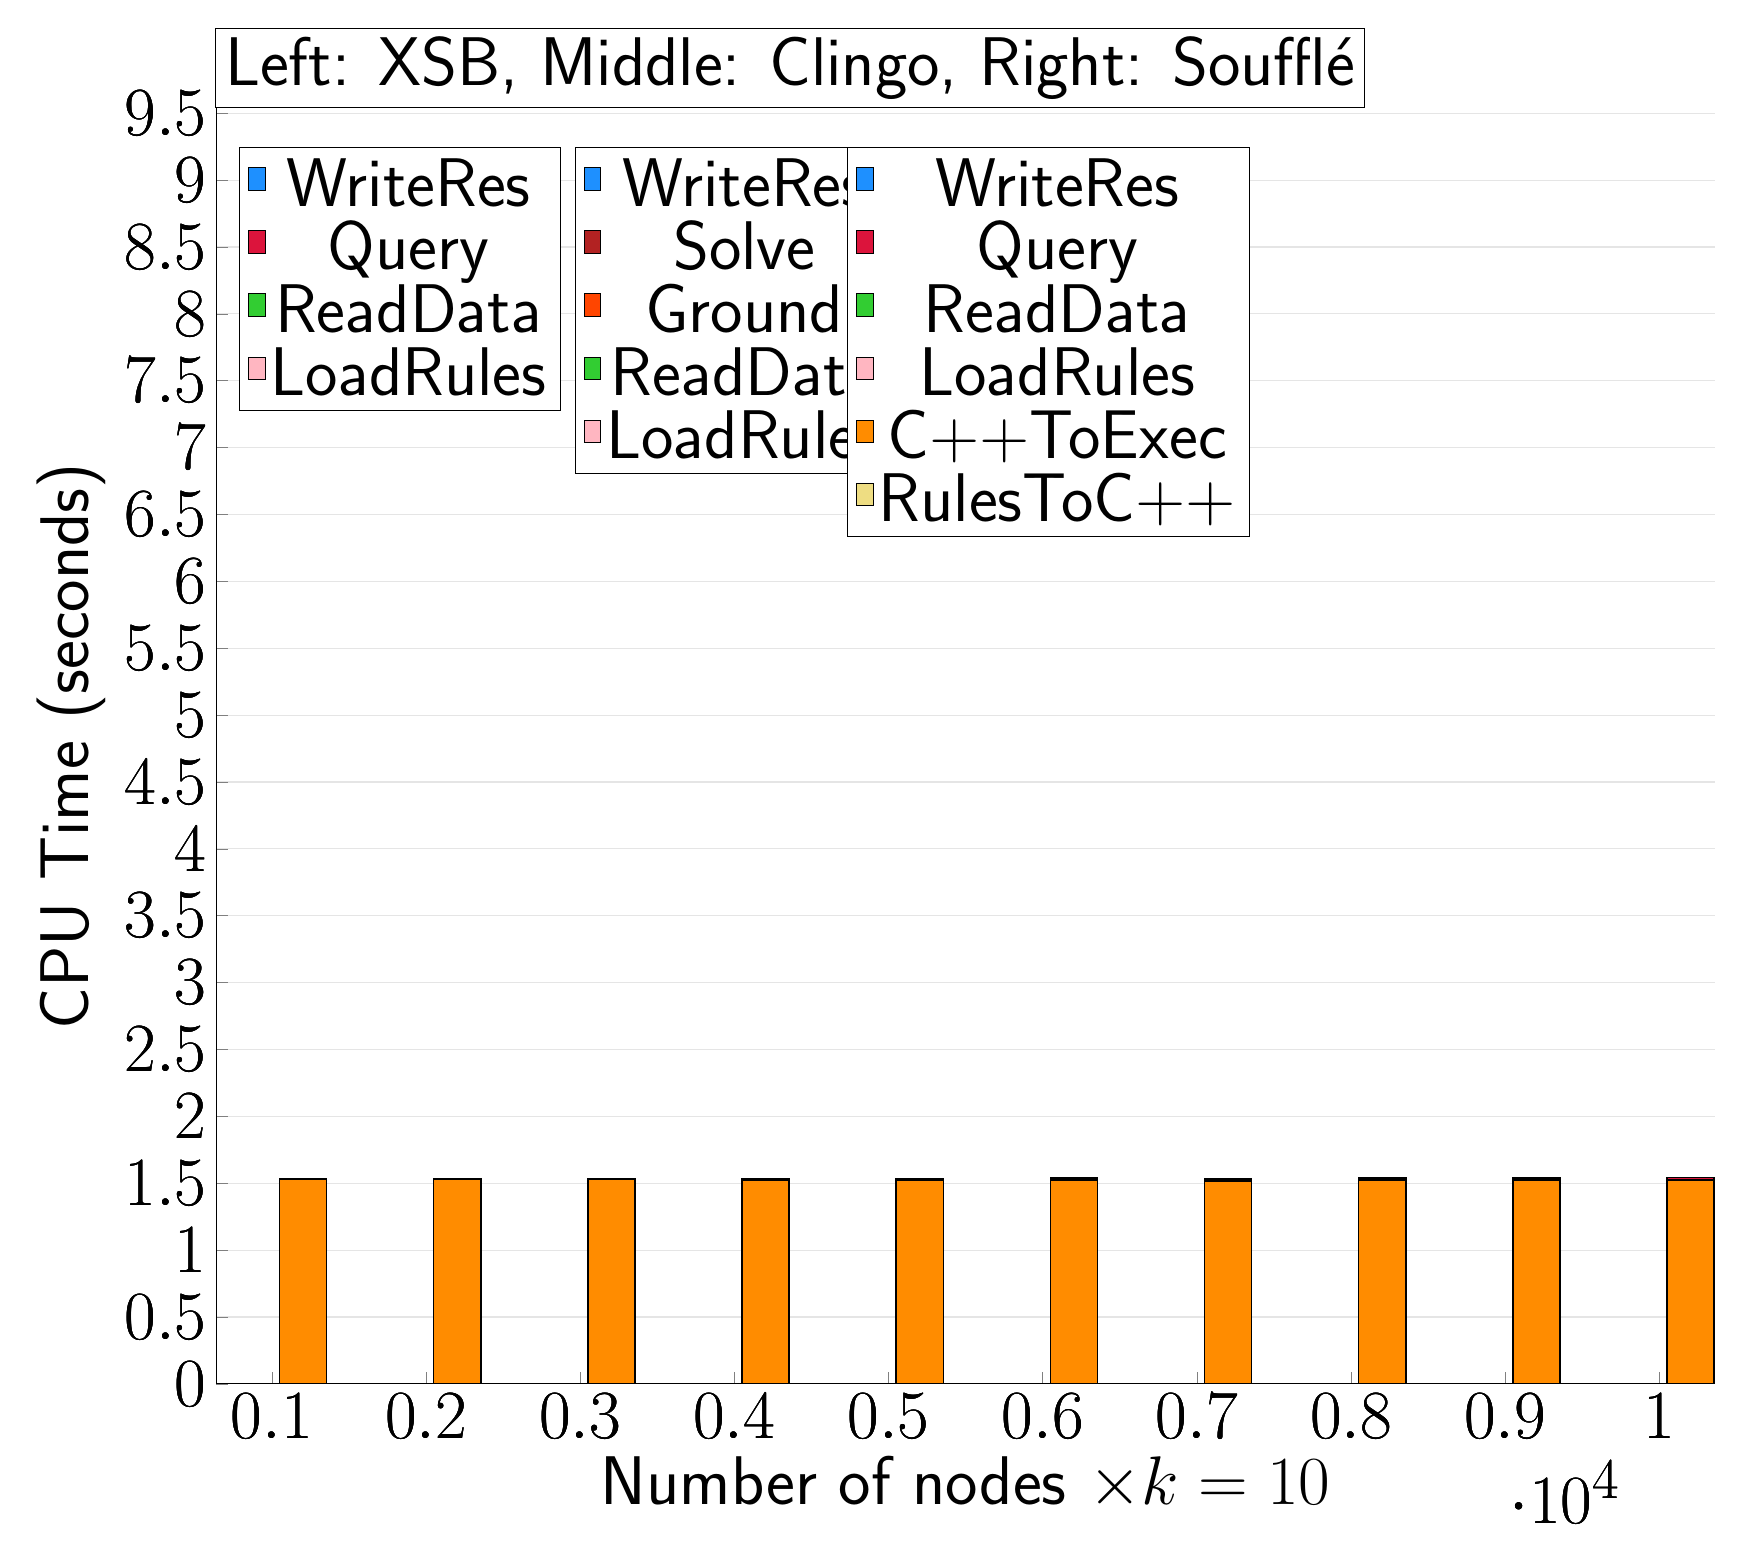
\begin{tikzpicture}
                        \begin{axis}[bar shift=-24.3pt, 
   ybar stacked,
   width=1.7\textwidth,
   bar width=0.6cm,
   ymajorgrids, tick align=inside,
   major grid style={draw=gray!20},
   xtick=data,
   ymin=0, ymax=9.536,
   axis x line*=bottom,
   axis y line*=left,
   enlarge x limits=0.04,
   legend style={
       at={(0.23, 0.97)},
       anchor=north east,
       legend columns=1,
       font=\Huge,
   },
   ylabel={CPU Time (seconds)},
   xlabel={Number of nodes $\times k=10$},
   label style={font=\Huge},
   tick label style={font=\Huge},
]
\addlegendimage{fill=DodgerBlue, draw=black, line width=0.2pt}
\addlegendentry{WriteRes}
\addlegendimage{fill=Crimson, draw=black, line width=0.2pt}
\addlegendentry{Query}
\addlegendimage{fill=LimeGreen, draw=black, line width=0.2pt}
\addlegendentry{ReadData}
\addlegendimage{fill=LightPink, draw=black, line width=0.2pt}
\addlegendentry{LoadRules}
\addplot +[fill=LightPink, draw=black, line width=0.55pt] coordinates {
(1000, 0.0005500000000000006)
(2000, 0.0005527999999999996)
(3000, 0.0005532000000000002)
(4000, 0.0005518000000000002)
(5000, 0.0005597999999999994)
(6000, 0.0005533999999999998)
(7000, 0.0005513999999999995)
(8000, 0.0005507999999999999)
(9000, 0.0005536)
(10000, 0.0005575999999999994)
};
\addplot +[fill=LimeGreen, draw=black, line width=0.55pt] coordinates {
(1000, 0.0002063999999999996)
(2000, 0.0002853999999999994)
(3000, 0.00036560000000000027)
(4000, 0.0004459999999999998)
(5000, 0.0005240000000000008)
(6000, 0.0006018000000000004)
(7000, 0.0006820000000000003)
(8000, 0.0007568)
(9000, 0.0008355999999999997)
(10000, 0.0009334000000000002)
};
\addplot +[fill=Crimson, draw=black, line width=0.55pt] coordinates {
(1000, 8.400000000000077e-06)
(2000, 8.600000000000617e-06)
(3000, 8.199999999999877e-06)
(4000, 9.000000000000671e-06)
(5000, 1.0200000000000136e-05)
(6000, 8.999999999999983e-06)
(7000, 9.200000000000183e-06)
(8000, 8.19999999999953e-06)
(9000, 8.79999999999978e-06)
(10000, 8.999999999999983e-06)
};
\addplot +[fill=DodgerBlue, draw=black, line width=0.55pt] coordinates {
(1000, 6.379999999999963e-05)
(2000, 6.439999999999915e-05)
(3000, 6.52000000000003e-05)
(4000, 6.439999999999881e-05)
(5000, 6.160000000000017e-05)
(6000, 6.399999999999944e-05)
(7000, 6.279999999999928e-05)
(8000, 6.400000000000048e-05)
(9000, 6.43999999999995e-05)
(10000, 6.35999999999994e-05)
};
\end{axis}

\begin{axis}[bar shift=-6.5pt, 
   ybar stacked,
   width=1.7\textwidth,
   bar width=0.6cm,
   ymajorgrids, tick align=inside,
   major grid style={draw=none},
   xtick=data,
   ymin=0, ymax=9.536,
   axis x line*=none,
   axis y line*=none,
   enlarge x limits=0.04,
   legend style={
       at={(0.454, 0.97)},
       anchor=north east,
       legend columns=1,
       font=\Huge,
   },
   label style={font=\Huge},
   tick label style={font=\Huge},
]
\addlegendimage{fill=DodgerBlue, draw=black, line width=0.2pt}
\addlegendentry{WriteRes}
\addlegendimage{fill=FireBrick, draw=black, line width=0.2pt}
\addlegendentry{Solve}
\addlegendimage{fill=OrangeRed, draw=black, line width=0.2pt}
\addlegendentry{Ground}
\addlegendimage{fill=LimeGreen, draw=black, line width=0.2pt}
\addlegendentry{ReadData}
\addlegendimage{fill=LightPink, draw=black, line width=0.2pt}
\addlegendentry{LoadRules}
\addplot +[fill=LightPink, draw=black, line width=0.55pt] coordinates {
(1000, 0.0)
(2000, 0.0)
(3000, 0.0)
(4000, 0.0)
(5000, 0.0)
(6000, 0.0)
(7000, 0.0)
(8000, 0.0)
(9000, 0.0)
(10000, 0.0)
};
\addplot +[fill=LimeGreen, draw=black, line width=0.55pt] coordinates {
(1000, 0.0)
(2000, 0.0)
(3000, 0.0)
(4000, 0.0)
(5000, 0.0)
(6000, 0.0)
(7000, 0.0)
(8000, 0.0)
(9000, 0.0)
(10000, 0.0)
};
\addplot +[fill=OrangeRed, draw=black, line width=0.55pt] coordinates {
(1000, 0.0)
(2000, 0.0)
(3000, 0.0)
(4000, 0.0)
(5000, 0.0)
(6000, 0.0)
(7000, 0.0)
(8000, 0.0020000000000000018)
(9000, 0.0020000000000000018)
(10000, 0.0040000000000000036)
};
\addplot +[fill=FireBrick, draw=black, line width=0.55pt] coordinates {
(1000, 0.0)
(2000, 0.0)
(3000, 0.0020000000000000018)
(4000, 0.0)
(5000, 0.0)
(6000, 0.0)
(7000, 0.0)
(8000, 0.0)
(9000, 0.0)
(10000, 0.0)
};
\addplot +[fill=DodgerBlue, draw=black, line width=0.55pt] coordinates {
(1000, 0.0)
(2000, 0.0)
(3000, -0.0020000000000000018)
(4000, 0.0)
(5000, 0.0)
(6000, 0.0)
(7000, 0.0)
(8000, 0.0)
(9000, 0.0)
(10000, 0.0)
};
\end{axis}

\begin{axis}[bar shift=11.3pt, 
   ybar stacked,
   width=1.7\textwidth,
   bar width=0.6cm,
   ymajorgrids, tick align=inside,
   major grid style={draw=none},
   xtick=data,
   ymin=0, ymax=9.536,
   axis x line*=none,
   axis y line*=none,
   enlarge x limits=0.04,
   legend style={
       at={(0.69, 0.97)},
       anchor=north east,
       legend columns=1,
       font=\Huge,
   },
   label style={font=\Huge},
   tick label style={font=\Huge},
]
\addlegendimage{fill=DodgerBlue, draw=black, line width=0.2pt}
\addlegendentry{WriteRes}
\addlegendimage{fill=Crimson, draw=black, line width=0.2pt}
\addlegendentry{Query}
\addlegendimage{fill=LimeGreen, draw=black, line width=0.2pt}
\addlegendentry{ReadData}
\addlegendimage{fill=LightPink, draw=black, line width=0.2pt}
\addlegendentry{LoadRules}
\addlegendimage{fill=DarkOrange, draw=black, line width=0.2pt}
\addlegendentry{C++ToExec}
\addlegendimage{fill=LightGoldenrod, draw=black, line width=0.2pt}
\addlegendentry{RulesToC++}
\addplot +[fill=LightGoldenrod, draw=black, line width=0.55pt] coordinates {
(1000, 0.0)
(2000, 0.0)
(3000, 0.0)
(4000, 0.0)
(5000, 0.0)
(6000, 0.0)
(7000, 0.0)
(8000, 0.0)
(9000, 0.0)
(10000, 0.0)
};
\addplot +[fill=DarkOrange, draw=black, line width=0.55pt] coordinates {
(1000, 1.532)
(2000, 1.53)
(3000, 1.528)
(4000, 1.526)
(5000, 1.52)
(6000, 1.524)
(7000, 1.516)
(8000, 1.522)
(9000, 1.52)
(10000, 1.5219999999999998)
};
\addplot +[fill=LightPink, draw=black, line width=0.55pt] coordinates {
(1000, 0.0001464)
(2000, 0.0001502)
(3000, 0.0001398)
(4000, 0.00016939999999999997)
(5000, 0.00014199999999999998)
(6000, 0.00014419999999999998)
(7000, 0.00015040000000000002)
(8000, 0.000149)
(9000, 0.00015199999999999998)
(10000, 0.0001356)
};
\addplot +[fill=LimeGreen, draw=black, line width=0.55pt] coordinates {
(1000, 0.0009328000000000001)
(2000, 0.0012326)
(3000, 0.0017984)
(4000, 0.002009)
(5000, 0.0023632)
(6000, 0.0028982)
(7000, 0.0031282)
(8000, 0.0033254)
(9000, 0.0038306)
(10000, 0.0042266)
};
\addplot +[fill=Crimson, draw=black, line width=0.55pt] coordinates {
(1000, 0.0024108000000000003)
(2000, 0.0038982)
(3000, 0.0062306)
(4000, 0.007298400000000001)
(5000, 0.009349600000000001)
(6000, 0.011556799999999999)
(7000, 0.0123466)
(8000, 0.0134568)
(9000, 0.016005600000000002)
(10000, 0.0177912)
};
\addplot +[fill=DodgerBlue, draw=black, line width=0.55pt] coordinates {
(1000, 0.000473)
(2000, 0.00030680000000000003)
(3000, 0.00033800000000000003)
(4000, 0.00030859999999999997)
(5000, 0.00030619999999999996)
(6000, 0.0002986)
(7000, 0.0002946)
(8000, 0.0002784)
(9000, 0.00028839999999999996)
(10000, 0.000255)
};
\end{axis}


\node[anchor=south, draw, fill=white] at (rel axis cs:0.42,1) {\Huge Left: XSB, Middle: Clingo, Right: Soufflé};
\end{tikzpicture}
\end{document}
                    